\documentclass[a4]{overview}
\title{Calculus Overview: Double Integral}

\tikzset{
  >={stealth}   % 设置全局默认箭头样式
}

\NewDocumentEnvironment{mathfig}{+b}
  {%
    \[
    \mathfigsplit#1\mathfigstop
    \]
  }
  {}

\long\def\mathfigsplit#1\tikzfig#2\mathfigstop{%
  \begin{aligned}
    #1
  \end{aligned}
  \quad
  \vcenter{\hbox{%
    \begin{tikzpicture}
      #2
    \end{tikzpicture}%
  }}%
}

\begin{document}
\maketitle

\section{Simple Double Integral}

\subsection{Linear Function}

\begin{theorem}
\[
	\iint_D x \dd x \dd y = \overline{x} A(D)
	\quad
	\iint_D y \dd x \dd y = \overline{y} A(D)
\] 
where $A(D)$ is the area of the domain $D$ and $\overline{x}$ and $\overline{y}$ are
the average values of $x$ and $y$ over the domain $D$. Or so called the geometric 
center of the domain $D$.

\end{theorem}

\section{Symmetry}

\begin{lemma}
Suppose a domain $D$ is described by constraints $D(x, y)$ denoting the equations or inequalities
that define the domain, we can define a new domain $D'(x, y) = D(y, x)$ by exchanging $x$ and $y$.
Then we have
\[
	\iint_D f(x, y) \dd \sigma = \iint_{D'} f(y, x) \dd \sigma
\] 
	
\end{lemma}

\begin{theorem}

When the domain $D$ is symmetric about the $y=x$, or in other words, exchanging
$x$ and $y$ does not change the domain, $D=D'$, then we have
\[
	\iint_D f(x, y) \dd \sigma = \iint_{D} f(y, x) \dd \sigma
	= \frac{1}{2} \iint_D \left[ f(x, y) + f(y, x) \right] \dd \sigma
\] 
\end{theorem}

\begin{example}
	\[
		I = \int_0^1 \dd x \int_{1-x}^{2-x} e^{(x+y)^2} (\sin^2 x + \cos^2 y) \dd y
		+\int_1^2 \dd x \int_{0}^{2-x} e^{(x+y)^2} (\sin^2 x + \cos^2 y) \dd y
	\] 
	\begin{answer}
		\begin{mathfig}
				I &= \iint_D e^{(x+y)^2} (\sin^2 x + \cos^2 y) \dd \sigma \\
				&= \frac{1}{2} \iint_D e^{(x+y)^2} (\sin^2 x + \cos^2 y + \sin^2 y + \cos^2 x) \dd \sigma \\
				&= \frac{1}{2} \iint_D e^{(x+y)^2} (1 + 1) \dd \sigma \\
				&= \iint_D e^{(x+y)^2} \dd \sigma
			\tikzfig
				% axis
				\draw[->] (-0.2,0) -- (2.5,0) node[right] {$x$};
				\draw[->] (0,-0.2) -- (0,2.5) node[above] {$y$};
				% x=1
				\draw[dashed] (1,0) -- (1,2.5);% node[right] {$x=1$};
				% y=2-x
				\draw[solid] (0,2) -- (2,0) node[above right] {$x+y=2$};
				% y=1-x
				\draw[solid] (0,1) -- (1,0) node[below right] {$x+y=1$};
				% domain
				% x 0 to 1
				\fill[cyan!30] (0,1) -- (0,2) -- (1,1) -- (1,0)  -- cycle;
				% x 1 to 2
				\fill[blue!20] (1,0) -- (1,1) -- (2,0) -- cycle;
				% symmetry line y=x
				\draw[red, dashed] (0,0) -- (2.5,2.5);
		\end{mathfig}
		Here we omit the details of the integral, which is not the focus of this example, 
		directly give the result for reference.
		\[
			I = \int_0^{\pi/2} \dd \theta \int_{1/(\cos \theta + \sin \theta)}
			^{2/(\cos \theta + \sin \theta)} e^{r^2} r \dd r
			= \frac{1}{2} e(e^{3}-1)
		\] 
	\end{answer}
\end{example}

\begin{lemma}

If the domain $D$ is symmetric about the line $y=x$, then we can divide the domain
into two parts $D_1$ and $D_2$ symmetrically,
(its arbitrary to choose which part is $D_1$ or $D_2$)

\begin{center}
\begin{tikzpicture}[scale=1.8, >=Latex]

% 坐标轴
\draw[->] (-0.4,0) -- (2.0,0) node[right] {$x$};
\draw[->] (0,-0.4) -- (0,2.0) node[above] {$y$};

% 对角线 y=x
\draw[red, thick] (0,0) -- (1.6,1.6) node[above right] {$y=x$};

% ===== 不规则曲线 C: y = f(x) =====
\draw[blue, thick, smooth]
plot coordinates {
    (0,1)
    (0.15,1.18)
    (0.35,1.05)
    (0.55,0.92)
    (0.75,0.85)
		(0.8,0.8)
};

% ===== 对称曲线 C': x = f(y)（即交换坐标）=====
\draw[blue, thick, smooth]
plot coordinates {
    (1,0)
    (1.18,0.15)
    (1.05,0.35)
    (0.92,0.55)
    (0.85,0.75)
		(0.8,0.8)
};

% 端点
\fill[blue] (0,1) circle (1pt);
\fill[blue] (1,0) circle (1pt);

% 标注
\node[red] at (0.7,0.3) {$D_1$};
\node[red] at (0.3,0.7) {$D_2$};


\end{tikzpicture}
\end{center}
then we have
\[
	\begin{aligned}
	\iint_D f(x, y) \dd \sigma
	&= \iint_{D_1} f(x, y) \dd \sigma + \iint_{D_2} f(x, y) \dd \sigma \\
	&= \iint_{D_1} f(x, y) \dd \sigma + \iint_{D_1} f(y, x) \dd \sigma \\
	&= \iint_{D_1} [f(x, y) + f(y, x)] \dd \sigma \\
	\end{aligned}
\] 
which is more convenient to calculate the integral since we only need to integrate
over half of the domain, dont need to consider piecewise boundary conditions.
	
\end{lemma}

\section{Polar Coordinates}

\[
\iint_D f(x, y) \dd x \dd y = \iint_D f(r \cos \theta, r \sin \theta) r \dd r \dd \theta
\] 

When $f$ contains $x^2 + y^2$, we can use the polar coordinates to simplify the $\theta$
since $x^2 + y^2 = r^2$. 
When $f$ is homogeneous, that 
we can

\subsection{Common Polar Regions}

\subsubsection{Eccentric circles}

There are two cases of common eccentric circles, both of them's center is on the
$x$ axis or $y$ axis, and pass through the origin. 
\[
	r = \pm \text{diameter} \cdot \sin \text{or} \cos \theta
\] 

\begin{center}
\begin{tikzpicture}[>=Stealth, scale=0.8]

\def\a{1.2} % 半径
\def\sep{6.2} % 两个图之间的水平间距

% 定义一个“上下两个圆”的图形
% #1：整体平移坐标
% #2: 第一个圆心坐标
% #3: 第二个圆心坐标
% #4: node direction
\newcommand{\twocircles}[4]{
\begin{scope}[shift={#1}]
    % 坐标轴
    \draw[->] (-3,0) -- (3,0) node[below] {$x$};
    \draw[->] (0,-2.8) -- (0,2.8) node[left] {$y$};

    % 上下两个圆
    \draw[blue] #2 circle (\a);
    \draw[cyan!70!blue] #3 circle (\a);

    % 圆心
    \fill #2  circle (1.2pt);
    \fill #3 circle (1.2pt);

    % 原点标记
    \node[below left] at (0,0) {$O$};

    % 标注 a, -a
    \node[#4] at #2 {$a$};
    \node[#4] at #3 {$-a$};
\end{scope}
}

\twocircles{(0,0)}{(\a,0)}{(-\a,0)}{below}
\twocircles{(\sep,0)}{(0,\a)}{(0,-\a)}{left}
% 公式标注
\node[blue] at (\a + .4,\a + .4) {$r=2a\cos\theta$};
\node[cyan!70!blue] at (-\a - .4,\a + .4) {$r=-2a\cos\theta$};

\node[blue, shift={(\sep, 0)}] at (\a + .5,\a) {$r=2a\sin\theta$};
\node[cyan!70!blue, shift={(\sep, 0)}] at (\a + .3,-\a - .7) {$r=-2a\sin\theta$};

\end{tikzpicture}
\end{center}

the derivation is simple, take x-axis as an example, the circle's equation
\[
	(x-a)^2 + y^2 = a^2 \iff x^2 + y^2 = 2ax
	\iff r^2 = 2ar\cos\theta \iff r = 2a\cos\theta
\] 

Inversely, this results gives us a way to find the graph of this kind of circle,
when we have a circle with polar equation $r = \pm 2a \cos\theta$ or $r = \pm 2a \sin\theta$, 
\begin{itemize}
	\item $\cos$ means the center is on the $x$ axis, $\sin$ means the center is on the $y$ axis.
	\item The sign of the equation indicates which side of the axis the center is located.
	\item  $a$ is the distance from the center to the origin, and also the radius of the circle.
\end{itemize}

\section{Coordinate Transformation}

Let $x = x(u, v)$ and $y = y(u, v)$ be a transformation from $(u, v)$ to $(x, y)$,
then we have
\[
	\iint_D f(x, y) \dd x \dd y = \iint_{D'} f(x(u, v), y(u, v)) 
	|J| \dd u \dd v
\] 
where $J$ is the Jacobian determinant of the transformation, defined as
\[
	J = \frac{\partial(x, y)}{\partial(u, v)} =
	\begin{vmatrix}
		x_u & x_v \\
		y_u & y_v
	\end{vmatrix}
\]
\begin{remark}
	Remember to change the domain $D$ to $D'$ when changing the variables, the new
	domain $D'$ is the region in the $uv$ plane that corresponds to the original region $D$ in the $xy$ plane
\end{remark}

\section{View another variable as a constant}

Sometimes, inner integral with another variable as parameter is very confusing,
hide that it maybe just a simple integral with parameter becomes a variable.

\begin{example}
	\[
		I = \int_0^1 \dd x \int_0^{x^2} \sqrt{x^{4} - y^2} \dd y
	\] 
	\begin{answer}
		Let $t=\sqrt{x^4 - y^2}$, then $t^2 + y^2 = x^4$, which is a circle with radius $x^2$.
		The inner integral is the area of a quarter circle.
		\[
			I = \int_0^1 \frac{\pi x^4}{4} \dd x
			= \frac{\pi}{20}
		\] 
	\end{answer}
\end{example}

\section{Change order of Iterated Integral}

When meeting a double integral with some obviously unable integrand function,
we always consider changing the order of integration, which may make the integral easier to calculate.
Here are some common cases of unable functions,
\begin{itemize}
	\item $\exp(\pm x^2), \exp(1 / x), 1 / \ln x$
	\item $\sin(x^2), \sin(1 / x), \sin x / x$
	\item $\cos(x^2), \cos(1 / x), \cos x / x$
	\item $\sqrt{x^{3}+1}, 1 / \sqrt{x^{3}+1}$
\end{itemize}

or very difficult to integrate functions
\begin{itemize}
	\item $\sqrt{a\pm x^2}$
\end{itemize}

\begin{example}
	\[
		I = \int_0^{\frac{\pi}{6}} \dd y \int_y^{\frac{\pi}{6}} \frac{\cos x}{x} \dd x
	\] 
\begin{answer}
	\[
		I = \int_0^{\frac{\pi}{6}} \dd x \int_0^x \frac{\cos x}{x} \dd y
		= \int_0^{\frac{\pi}{6}} \cos x \dd x
		= \frac{1}{2}
	\] 
	
\end{answer}
	
\end{example}

\begin{example}
	\[
		I = \int_0^{\infty} \dd y \int_y^{2y} e^{-x^2} \dd x
	\]
\begin{answer}
	\begin{mathfig}
		I &= \int_0^{\infty} \dd x \int_{\frac{x}{2}}^x e^{-x^2} \dd y \\
			&= \int_0^{\infty} \frac{x}{2} e^{-x^2} \dd x \\
			&= -\frac{1}{4} \int_0^{\infty} e^{-x^2} \dd (e^{-x^2})\
			= \frac{1}{4} \\
	\tikzfig
		% axis
		\draw[->] (-0.2,0) -- (3,0) node[right] {$x$};
		\draw[->] (0,-0.2) -- (0,3) node[above] {$y$};

		% x=y
		\draw[dashed] (0,0) -- (2.4,2.4) node[above] {$x=y$};
		% x=2y
		\draw[dashed] (0,0) -- (3,1.5) node[right] {$x=2y$};

		% domain
		\fill[blue!20] (0,0) -- (2.4,2.4) -- (3,1.5) -- cycle;

		% fix x to get the limits of y
		\draw[->, red] (1.5, .75) -- (1.5, 1.5) node[above] {$y \in [\frac{x}{2}, x]$};
	\end{mathfig}
\end{answer}
	
\end{example}

When changing the order of integration, we need to pay attention to the upper and
lower limits, when upper limit is less than lower limit, its easy to make mistakes,
so we recommend always to extract the negative sign and change the order of the limits,
to \textbf{make lower limit less than upper limit.}

\begin{example}
	\[
		I = \int_0^1 \dd x \int_1^x \frac{\tan y}{y} \dd y
	\]
\begin{answer}
	\begin{mathfig}
		I &= -\int_0^1 \frac{\tan y}{y}\dd y \int_0^y \dd x  \\
			&= -\int_0^1 \tan y \dd y \\
			&= \ln \cos 1
	\tikzfig[scale=2]
	% axis
	\draw[->] (-0.2,0) -- (1.5,0) node[right] {$x$};
	\draw[->] (0,-0.2) -- (0,1.5) node[above] {$y$};

	% x=1
	\draw[dashed] (1,0) -- (1,1.5) node[right] {$x=1$};
	% y=1
	\draw[dashed] (0,1) -- (1.5,1) node[above] {$y=1$};
	% y=x
	\draw[dashed] (0,0) -- (1.5,1.5) node[above right] {$y=x$};

	% domain
	\fill[blue!20] (0,0) -- (1,1) -- (0,1) -- cycle;
	\node[blue] at (.33,.66) {$D$};

	% fix y to get the limits of x
	\draw[->, red] (0, .8) -- (.8, .8) node[right] {$x \in [0, y]$};
	\end{mathfig}
\end{answer}
\end{example}

\subsection{Special Case For Inverse Trigonometric Functions}

For inverse trigonometric functions, $\asin$ and $\acos$ has principal value range
\[
	\asin x \in [-\frac{\pi}{2}, \frac{\pi}{2}]
	\quad
	\acos x \in [0, \pi]
\]

\begin{center}
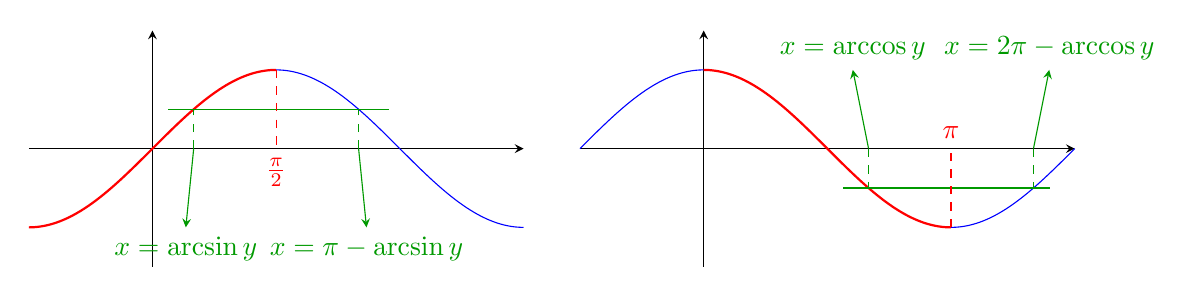
\begin{tikzpicture}[samples=80]

%==================== 左图：arcsin ====================
\begin{scope}[xshift=0cm]

% 坐标轴
\draw[->] (-pi/2,0) -- (3*pi/2,0);
\draw[->] (0,-1.5) -- (0,1.5);

% sin 曲线（分段上色）
\draw[thick, red, domain=-pi/2:pi/2, smooth, variable=\x]
    plot ({\x},{sin(\x r)});
\draw[blue, domain=pi/2:3*pi/2, smooth, variable=\x]
    plot ({\x},{sin(\x r)});

% 水平参考线 y = 0.5
\draw[green!60!black] (.2,0.5) -- (3,0.5);

% x = arcsin(0.5)
\draw[dashed, green!60!black] ({pi/6},{0}) -- ({pi/6},{0.5});
\draw[->, green!60!black] (pi/6,0) -- (pi/6 - .1,-1) node[below]{$x=\arcsin y$};

% x = π - arcsin(0.5)
\draw[dashed, green!60!black] ({5*pi/6},{0}) -- ({5*pi/6},{0.5});
\draw[->, green!60!black] (5*pi/6,0) -- (5*pi/6 + .1,-1) node[below]{$x=\pi-\arcsin y$};

% π/2 标记
\draw[dashed, red] ({pi/2},1) -- ({pi/2},0);
\node[red] at (pi/2,-0.3) {$\frac{\pi}{2}$};

\end{scope}

%==================== 右图：arccos ====================
\begin{scope}[xshift=7cm]

% 坐标轴
\draw[->] (-pi/2,0) -- (3*pi/2,0);
\draw[->] (0,-1.5) -- (0,1.5);

% cos 曲线（分段上色）
\draw[blue, domain=-pi/2:0, smooth, variable=\x]
    plot ({\x},{cos(\x r)});
\draw[thick,red, domain=0:pi, smooth, variable=\x]
    plot ({\x},{cos(\x r)});
\draw[blue, domain=pi:3*pi/2, smooth, variable=\x]
    plot ({\x},{cos(\x r)});

% 水平参考线 y = -0.5
\draw[green!60!black] (pi/2+.2,-0.5) -- (4.4,-0.5);

% x = arccos(-0.5)
\draw[dashed, green!60!black] ({2*pi/3},{0}) -- ({2*pi/3},{-0.5});
\draw[->, green!60!black] (2*pi/3,0) -- (2*pi/3 - .2,1) node[above]{$x=\arccos y$};

% x = 2π - arccos(-0.5)
\draw[dashed, green!60!black] ({4*pi/3},{0}) -- ({4*pi/3},{-0.5});
\draw[->, green!60!black] (4*pi/3,0) -- (4*pi/3 + .2,1) node[above]{$x=2\pi-\arccos y$};

% π 标记
\draw[dashed, red] ({pi},-1) -- ({pi},0) node[above] {$\pi$};

\end{scope}
\end{tikzpicture}
\end{center}

To find actual inverse value, we first find the principal pos, then use
the symmetry of the function to find the actual value.

\subsection{Change of order in polar coordinates}

When changing the order of integration in polar coordinates, in order to determine
the region of integration, there are two common methods, one is to directly
analyze the region in polar coordinates draw in xOy plane.

Then to get the limits, we fix $r$ draw a circle with radius $r$, then find the
intersection points with the boundary of the region, so that find the limits of
 $\theta$ for the fixed $r$.

Another is to consider
$r, \theta$ as perpendicular coordinates, then tackle as the rectangular coordinates
which is similar to the $xOy$ plane. 

\begin{example}
	\[
		I = \int_0^{2\pi} \dd \theta \int_{\theta /2}^{\pi} \theta^2 e^{r^2} \dd r
	\] 

\begin{answer}
	\[
		\begin{aligned}
			I &= \int_0^{\pi} \dd r \int_0^{2r} \theta^2 e^{r^2} \dd \theta
			 = \int_0^{\pi} e^{r^2} \dd r \frac{1}{3} (2r)^3
			 = \frac{8}{3} \int_0^{\pi} r^3 e^{r^2} \dd r
			  = \frac{4}{3} e^{\pi^2} (\pi^2 - 1) + \frac{4}{3}
			 
		\end{aligned}
	\] 
\begin{center}
%Method 1
	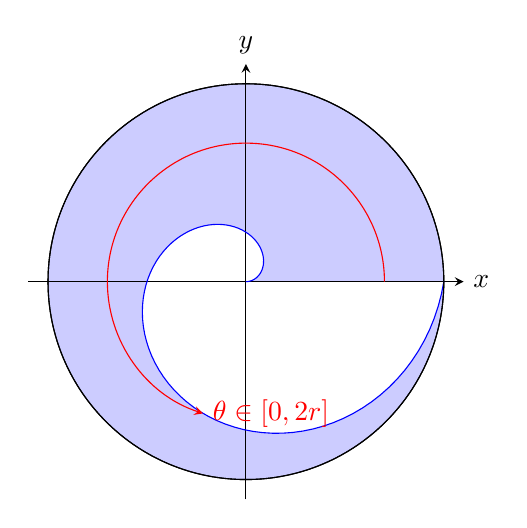
\begin{tikzpicture}[baseline=(current bounding box.center),scale=0.8]
	% domain
	\fill[blue!20, domain=2*pi:0, samples=100, variable=\t]
			(0,0) -- (pi,0)
			arc[start angle=0,end angle=360,radius=pi]
			plot ({0.5*\t*cos(\t r)}, {0.5*\t*sin(\t r)})
			-- cycle;
	% axis
	\draw[->] (-1.1*pi, 0) -- (1.1*pi,0) node[right] {$x$};
	\draw[->] (0,-1.1*pi) -- (0,1.1*pi) node[above] {$y$};

	% r=pi
	\draw[] (pi,0) arc (0:360:pi);
	% theta=2r
	\draw[domain=0:2*pi, samples=100,  variable=\t, blue]
			plot ({0.5*\t*cos(\t r)}, {0.5*\t*sin(\t r)});
	\draw[] (pi,0) arc (0:360:pi);
	\draw[->,red] (.7*pi,0) arc (0:1.4*pi r:.7*pi) node [above,right] {$\theta \in [0, 2r]$};
\end{tikzpicture}
%Method 2
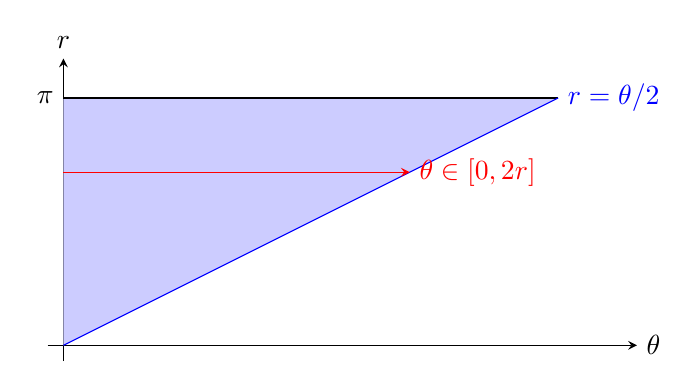
\begin{tikzpicture}[baseline=(current bounding box.center)]
	% axis
	\draw[->] (-0.2,0) -- (2*pi+1,0) node[right] {$\theta$};
	\draw[->] (0,-0.2) -- (0,pi+.5) node[above] {$r$};

	% domain
	\fill[blue!20] (0,0) -- (2*pi,pi) -- (0, pi) -- cycle;
	% r=pi
	\draw[] (0,pi) -- (2*pi,pi) node[at start, left] {$\pi$};
	% theta=2r
	\draw[blue] (0,0) -- (2*pi,pi) node[right] {$r=\theta/2$};
	% fix r
	\draw[->,red] (0, 0.7*pi) -- (1.4*pi, 0.7*pi) node[right] {$\theta \in [0, 2r]$};

\end{tikzpicture}
\end{center}
	
\end{answer}
\end{example}
	

\end{document}
